\documentclass{beamer}
\usetheme{Boadilla}
\usepackage{hyperref}
\usepackage{graphicx}
\usepackage{fancyvrb}
\usepackage{multicol}
\usepackage{subfig}
\usepackage[
    backend=biber, 
    natbib=true,
    style=numeric,
    sorting=none,
    style=verbose-ibid,
]{biblatex}
\addbibresource{citations.bib}
\usepackage{pgfpages}
\usepackage{xcolor}
\definecolor{ao(english)}{rgb}{0.0, 0.5, 0.0}
\definecolor{burgundy}{rgb}{0.5, 0.0, 0.13}
%\setbeameroption{show notes}
\setbeameroption{show notes on second screen=right}
%\setbeameroption{hide notes}

\title{Gabor's 1946 Theory of Communication}
\author{Sevag Hanssian}
\institute{MUMT 622, Winter 2021}
\setbeamertemplate{navigation symbols}{}

\begin{document}

\begin{frame}
\maketitle
\end{frame}

\begin{frame}
	\frametitle{Significance}
	Outcomes of Gabor's 1946 paper, ``Theory of Communication''\footfullcite{gabor1946}:
	\vspace{0.5em}
	\begin{enumerate}
		\item
			First introduction of the time-frequency uncertainty principle, leading to an explosion of wavelet research in the 80s\footfullcite{homage1}
		\item
			Proposed that any signal of finite energy can be decomposed into a linear combination of time-frequency shifts of the Gaussian function\footfullcite{gaborwrong}
		\item
			First use of the STFT, or the windowed Fourier transform with Gaussian windows\footfullcite{textbook1}
		\item
			Showed that Gaussian-windowed STFT minimizes time-frequency uncertainty
	\end{enumerate}
\end{frame}

\begin{frame}
	\frametitle{Heisenberg's Uncertainty Principle}
	Heisenberg's uncertainty principle in quantum physics\footfullcite{hallm}:
	    \[ \sigma_{x}\sigma_{p} \ge \frac{h}{4\pi} \]
	    Heisenberg, 1927:
	    \begin{quote}
		    the more precisely the position [of an electron] is determined, the less precisely the momentum is known, and conversely
	    \end{quote}
\end{frame}

\note{
	\begin{itemize}
		\item
			in the world of quantum physics this is a core of the Copenhagen school, which Einstein disagreed with. this seems to be a fundamental limitation of the universe (as far as we know it)
	\end{itemize}
}

\begin{frame}
	\frametitle{Gabor's Uncertainty Principle}
	Gabor's time-frequency uncertainty:
	    \[ \sigma_{t}\sigma_{f} \ge \frac{1}{4\pi},\qquad\Delta t\Delta f \ge 1 \]
	    Gabor, 1946\footfullcite{gabor1946}:
	    \begin{quote}
		    although we can carry out the analysis [of the acoustic signal] with any degree of accuracy in the time direction or frequency direction, we cannot carry it out simultaneously in both beyond a certain limit
	    \end{quote}
\end{frame}

\note{
	\begin{itemize}
		\item
			Gabor says delta f and delta t are the uncertainties inherent in the definition of the epoch t and frequency f of an oscillation
		\item
			Just to super emphasize, this is a property of our choice to use the linear Fourier transform. it's not an inherent aspect of acoustic waves or signals, just our choice
		\item
			This is a consequence of the Fourier transform, as can be seen in the Flandrin textbook (pointed out by our prof)
		\item
			in quantum terms, t and f are conjugate variables, they are Fourier transform duals
	\end{itemize}
}

\begin{frame}
	\frametitle{Time-frequency tradeoff, intuition}
	\begin{figure}
		\centering
		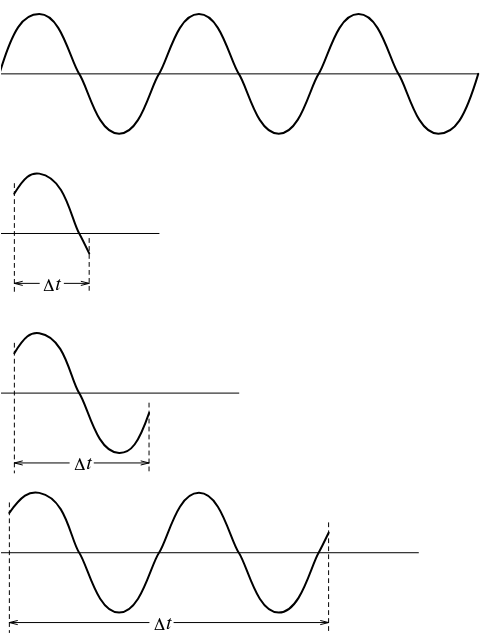
\includegraphics[height=5cm]{./gabor2.png}
		\caption{Improved frequency measurement over longer time intervals. The uncertainty in the frequency $\Delta f$ decreases as the measurement interval $\Delta t$ increases and vice versa\footfullcite{gabor2}}
	\end{figure}
\end{frame}

\begin{frame}
	\frametitle{Gabor's Uncertainty Principle, visual}
	\begin{figure}
		\centering
		\subfloat{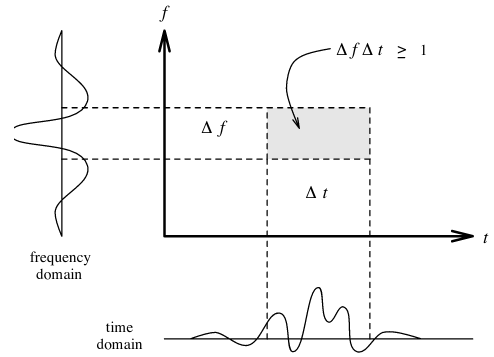
\includegraphics[height=4cm]{./tf-resolution2.png}}
		\hspace{0.35em}
		\subfloat{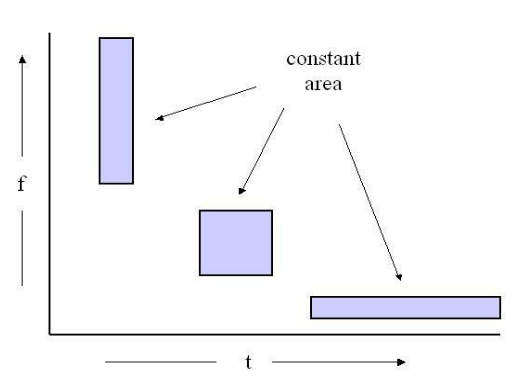
\includegraphics[height=4cm]{./tf-resolution.png}}
		\caption{The most a signal can be localized in the Fourier domain is into rectangles of size $\Delta t\Delta f = 1$}
	The smallest possible $\Delta t \Delta f$ rectangle is called the \textit{logon}, a ``unit of information''
	\end{figure}
\end{frame}

\begin{frame}
	\frametitle{Consequence of the Fourier transform}
	\begin{quote}
	In time-frequency analysis, it has been proven that linear operators cannot exceed the uncertainty bound [...] Nonlinearity does not by itself confer any acuity advantage, and in fact most nonlinearities are merely distortions and thus deleterious. However, by the above theorem, any carefully crafted analysis that can beat this limit must necessarily be nonlinear.\footfullcite{psycho}
	\end{quote}
\end{frame}

\begin{frame}
	\frametitle{Time-frequency tradeoff, visual}
	Arises from the linearity of the Fourier transform
	\begin{figure}
		\centering
		\subfloat[Unit impulse vs. infinite sine wave\footfullcite{gabor1946}]{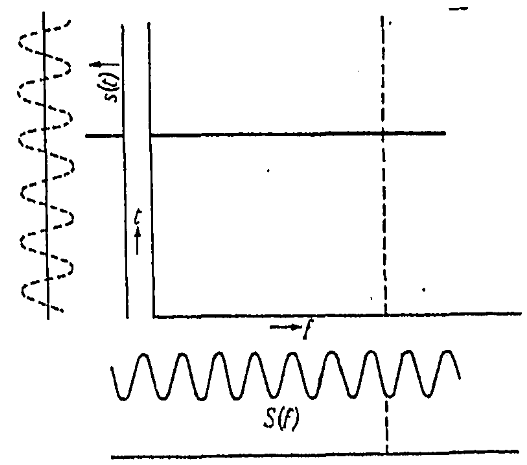
\includegraphics[width=4cm]{./gabor1.png}}
		\hspace{0.2em}
		\subfloat[Spread of a signal and its Fourier transform are inversely proportional\footfullcite{gabor2}]{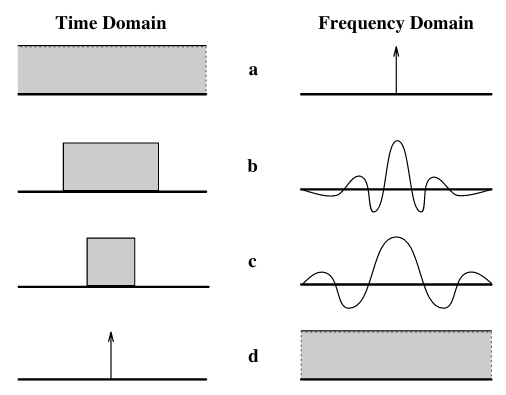
\includegraphics[width=5cm]{./gabor3.png}}
		\caption{Time vs. frequency}
	\end{figure}
\end{frame}

\begin{frame}
	\frametitle{Physical intuitions}
	\begin{quote}
		The foregoing solutions [of the Fourier transform], though unquestionably mathematically correct, are somewhat difficult to reconcile with our physical intuitions and our physical concepts of such variable frequency mechanisms as, for instance, the siren
	\end{quote}
	-- Carson (quoted by Gabor)
	\begin{quote}
	\vspace{2em}
		Gabor came to the conclusion that the difficulty lay in our mutually exclusive formulations of time analysis and frequency analysis ... he suggested a new method of analyzing signals in which time and frequency play symmetrical parts.\footfullcite{korpel}
	\end{quote}
\end{frame}

\note{
	\begin{itemize}
		\item
			this points to the origin of the wavelet and searching for alternative, non-linear representations of time-domain signals
	\end{itemize}
}

\begin{frame}
	\frametitle{Psychoacoustics}
	Psychoacoustic\footfullcite{psycho} studies have shown that humans can exhibit a better time-frequency resolution than Gabor's limit:
	\begin{quote}
		We have conducted the first direct psychoacoustical test of the Fourier uncertainty principle in human hearing, by measuring simultaneous temporal and frequency discrimination. Our data indicate that human subjects often beat the bound prescribed by the uncertainty theorem, by factors in excess of 10.
	\end{quote}
	Similarly to how Gabor was dissatisfied with time-frequency's inability to reconcile with physical intuitions:
	\begin{quote}
		most sound analysis and processing tools today continue to use models based on spectral theories. We believe it is time to revisit this issue.
	\end{quote}
\end{frame}

\note{
	\begin{itemize}
		\item
			In fact its not a defeat of Gabor, its a justification that we need to find better representations -- it actually supports the search for decompositions with non-linear components
	\end{itemize}
}

\begin{frame}
	\frametitle{Psychoacoustics}
	Brian C. J. Moore in 1973:\footfullcite{moore}
	\begin{quote}
		It is concluded that models based on a place (spectral) analysis should be subject to a limitation of the type $\Delta f \cdot d \ge \text{constant}$, where $\Delta f$ is the frequency difference limen (DL) for a tone pulse of duration d. [...]  It was found that at short durations the product of $\Delta f$ and d was about one order of magnitude smaller than the minimum predicted from the place model
	\end{quote}
\end{frame}

\note{
	\begin{itemize}
		\item
			frequency difference limen is similar to JND
		\item
			Consider that some psychoacoustic theories of hearing state that the cochlea does a tonotopic spectral decomposition, making it subject to the limitation
	\end{itemize}
}

\begin{frame}
	\frametitle{Gabor elementary functions}
	\begin{quote}
		What is the shape of the signal for which the product $\Delta t\Delta f$ actually assumes the smallest possible value? [... it is] the  modulation product of a harmonic oscillation of any frequency with a pulse of the form of the probability function
	\end{quote}
	i.e. apply a Gaussian envelope to the signal\\
	\[ \psi(t) = \text{e}^{-\alpha^{2}(t-t_{0})}\text{cis}(2\pi f_{0}t + \phi) \]
	\[ \phi(f) = \text{e}^{-\frac{\pi}{\alpha}^{2}(f-f_{0})^{2}}\text{cis}[-2\pi(f - f_{0}) + \phi)] \]
	The constant $\alpha$ is connected with $\Delta t$ and $\Delta f$ as follows:
	\[ \Delta t = \sqrt{\frac{\pi}{2}}\frac{1}{\alpha}, \Delta f = \frac{1}{\sqrt{2\pi}}\alpha \]
\end{frame}

\note{
	\begin{itemize}
		\item
			probability function = Gaussian
		\item
			Gaussian envelope of the finite-duration time signal
	\end{itemize}
}

\begin{frame}
	\frametitle{Gabor elementary functions, alternative form}
	Alternate form in \cite{gabor2}:\\\ \\
	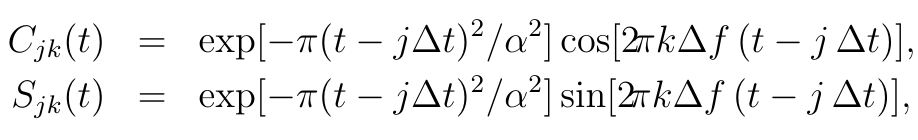
\includegraphics[width=8cm]{./gaboralt1.png}\\
	\vspace{-0.5em}
	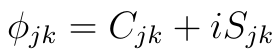
\includegraphics[width=2.5cm]{./gaboralt2.png}\\
	As $\alpha \rightarrow \infty$, this reduces to the Fourier representation:
	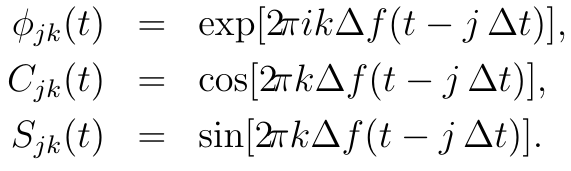
\includegraphics[width=5cm]{./gaboralt3.png}\\
	As $\alpha \rightarrow 0$, this reduces to Dirac delta functions spaced at $\Delta t$:
	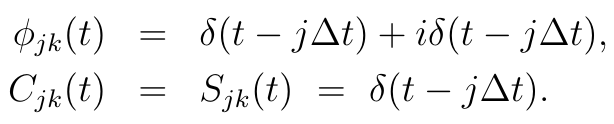
\includegraphics[width=5cm]{./gaboralt4.png}
\end{frame}

\note{
	\begin{itemize}
		\item
			absolute localization in frequency, no time information
		\item
			absolute localization in time, no frequency information
	\end{itemize}
}

\begin{frame}
	\frametitle{Gabor elementary functions}
	The parameter $\alpha$ determines the locality (spread) of the Gaussian envelope
	\begin{figure}
		\centering
		\subfloat[Envelope of the elementary signal]{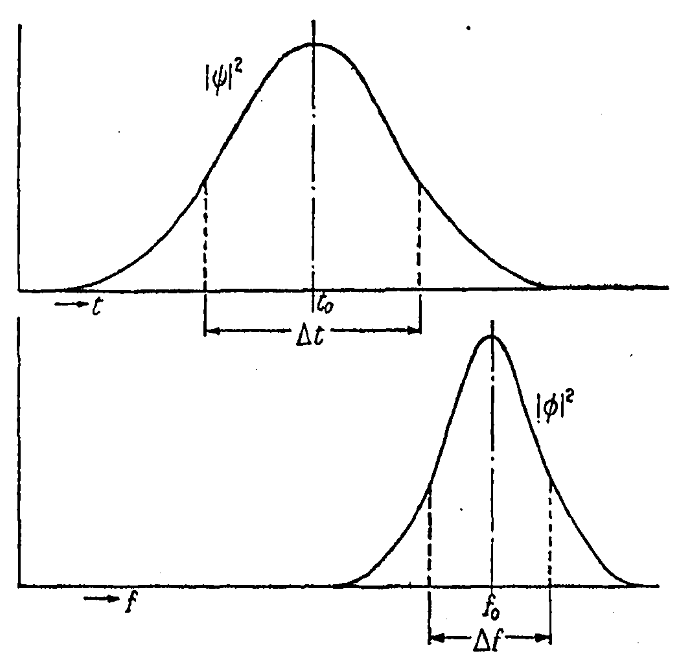
\includegraphics[height=4cm]{./gabor4.png}}
		\hspace{0.2em}
		\subfloat[Unit impulse vs. infinite sine wave]{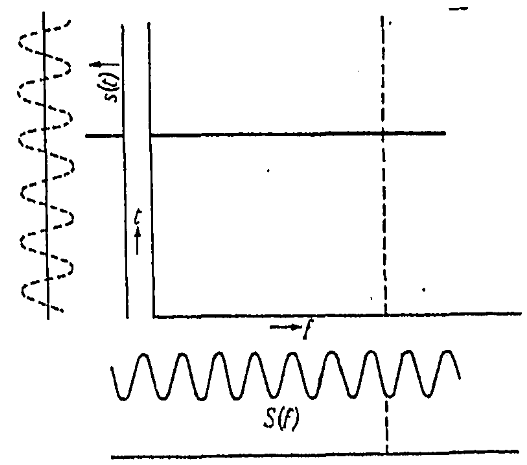
\includegraphics[width=4.5cm]{./gabor1.png}}
		\caption{Limits of $\alpha$ result in an ``impulse'' in time and frequency\footfullcite{gabor1946}}
	\end{figure}
\end{frame}

\begin{frame}
	\frametitle{Relation to Shannon's 1948 Sampling Theorem}
	Most important outcome of Shannon's seminal communications paper\footfullcite{shannon1948} in 1948, the Sampling Theorem, states that ``to reconstruct $\psi$ we must take equally spaced samples at a minimum of the Nyquist frequency, which is twice the maximal frequency''\footfullcite{gabor2}\\
	Recall that in Gabor's representation, as $\alpha \rightarrow 0$, this reduces to Dirac delta functions spaced at $\Delta t$:\\
	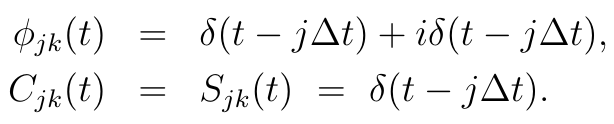
\includegraphics[width=5cm]{./gaboralt4.png}\\
	The $\alpha = 0$ limit represents two samples, $a_{jk}, b_{jk}$ for each $\Delta t$ interval, as required by Shannon's Sampling Theorem.
\end{frame}

\note{
	\begin{itemize}
		\item
			this is the simpler of the two, read full paper for the other
	\end{itemize}
}

\begin{frame}
	\frametitle{Gaussian window}
	\begin{figure}
		\centering
		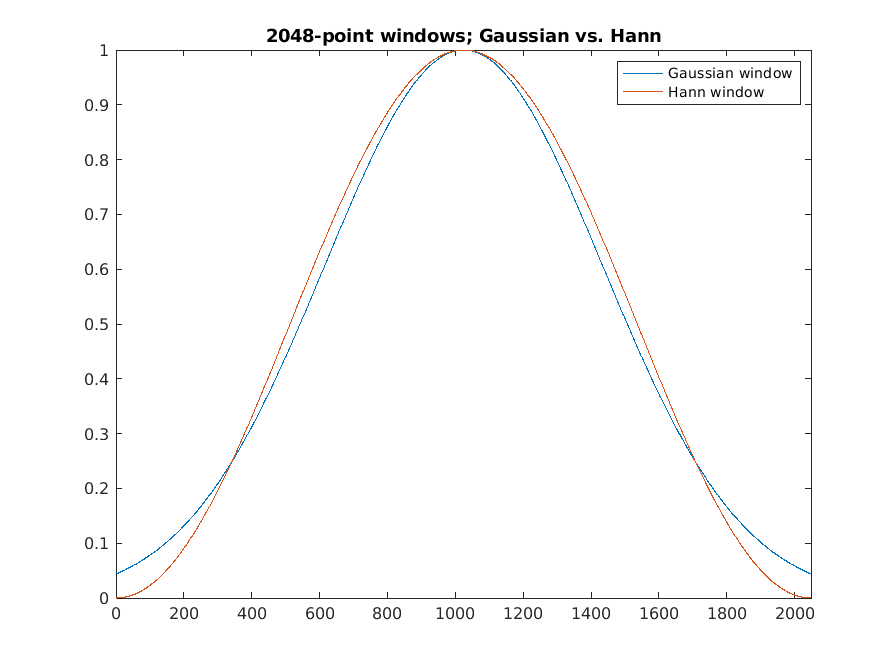
\includegraphics[width=7cm]{./gaussianvshann.png}
		\caption{gausswin and hann windows in MATLAB}
	\end{figure}
	Note that Hann window is exactly 0 outside of the specified range\\
	Gaussian asymptotically approaches 0 but never reaches it
\end{frame}

\begin{frame}
	\frametitle{Problems with the Gabor functions}
	Summarized from \cite{gabor2}
	\begin{enumerate}
		\item[1]
			The Gabor functions are \textbf{not strictly local} -- along with their infinite Gaussian envelope, they stretch out to infinity\\
			Biologically problematic, but the Gaussian envelope is well-localized (99.7\% of its area is within 3 standard deviations of the mean), so can be a ``good enough approximation'' of biology
		\item[2]
			The Gabor representation is \textbf{nonorthogonal}. This means computing the coefficients is \textit{possible} but not with the simple inner product. Inner products can lead to a good estimation of the Gabor coefficients with iterative refinement (Daugman's 1993 algorithm\footfullcite{daugman1993})
	\end{enumerate}
	Daugman unified Gabor elementary functions and wavelets by defining Gabor wavelets
\end{frame}

\begin{frame}
	\frametitle{Problems with the Gabor functions}
	\begin{enumerate}
		\item[3]
			Despite being nonorthogonal in $L_{2}(\mathbb{R})$, they can \textbf{still be a frame}\footfullcite{walnut}
			\begin{quote}
			However, the requirements of orthogonality and the basis property are very stringent, making it difficult as a rule to find a good orthonormal basis. As an alternative to orthonormal bases, we present a generalization known as frames. 
			\end{quote}
			Also:
			\begin{quote}
				Nonorthogonality is ubiquitous in biological systems -- we should learn how nature lives with it and even exploits it'' [...] orthogonality is a rather delicate property -- functions either are or aren't orthogonal; there are no degrees of orthogonality -- and so it is probably too fragile for biology to be able to depend on it.
			\end{quote}
	\end{enumerate}
\end{frame}

\begin{frame}
	\frametitle{Problems with the Gabor functions}
	\cite{gaborwrong} for further reading
	\begin{quote}
		In 1932 John von Neumann conjectured without proof that the time-frequency shifts of the Gaussian span a dense subspace in the space of signals of finite energy. In 1946 Gabor conjectured that the time-frequency shifts of the Gaussian is a basis for the space of signals of finite energy. [...] In colloquial terms, the expansions are numerically unstable and cannot be used in practice.
	\end{quote}
\end{frame}

\begin{frame}
	\frametitle{Time-frequency resolution in the STFT}
	Using default MATLAB spectrogram parameters\footfullcite{matlabspecgram} (Hamming window)
	\begin{figure}
		\vspace{-1em}
		\centering
		\subfloat[Good $\Delta t$, bad $\Delta f$]{{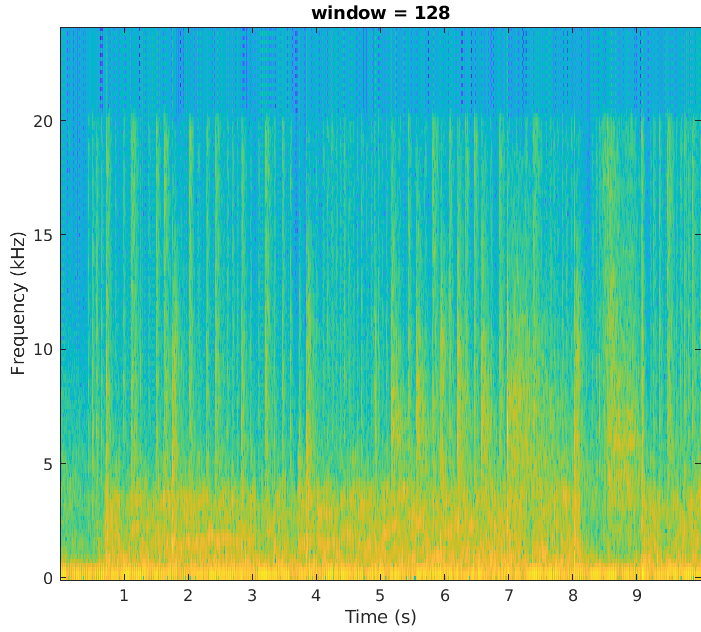
\includegraphics[width=5cm]{./stft_small.png} }}
		\subfloat[Good $\Delta f$, bad $\Delta t$]{{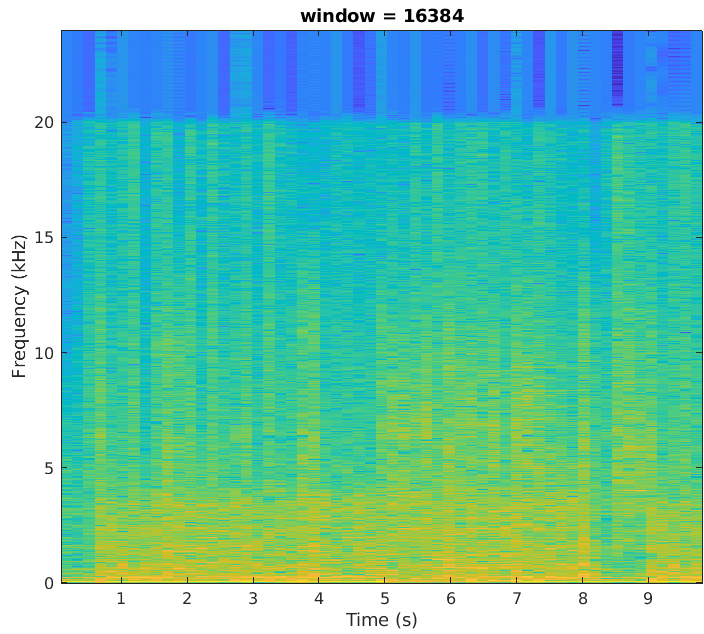
\includegraphics[width=5cm]{./stft_big.png} }}
		\caption{STFT, small vs. big window}
	\end{figure}
\end{frame}

\begin{frame}
	\frametitle{Time-frequency resolution in the STFT}
	\begin{figure}
		\centering
		\subfloat[Good $\Delta t$, bad $\Delta f$]{{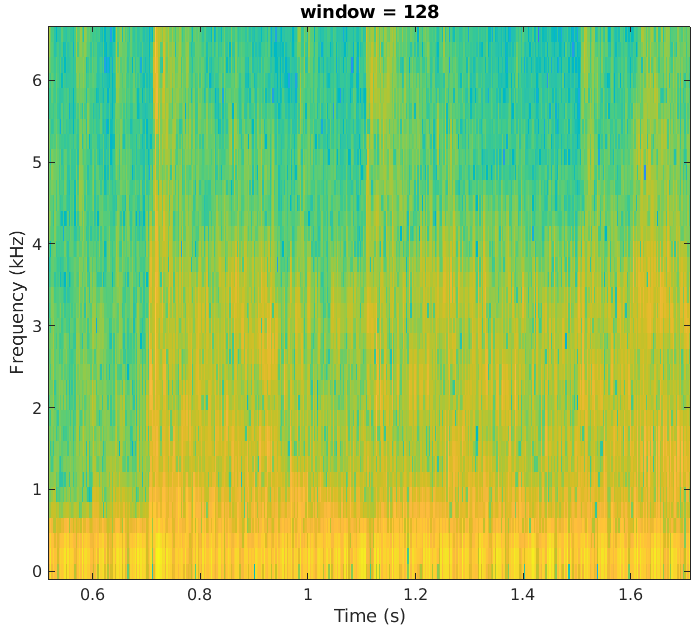
\includegraphics[width=5cm]{./stft_small_zoomed.png} }}
		\subfloat[Good $\Delta f$, bad $\Delta t$]{{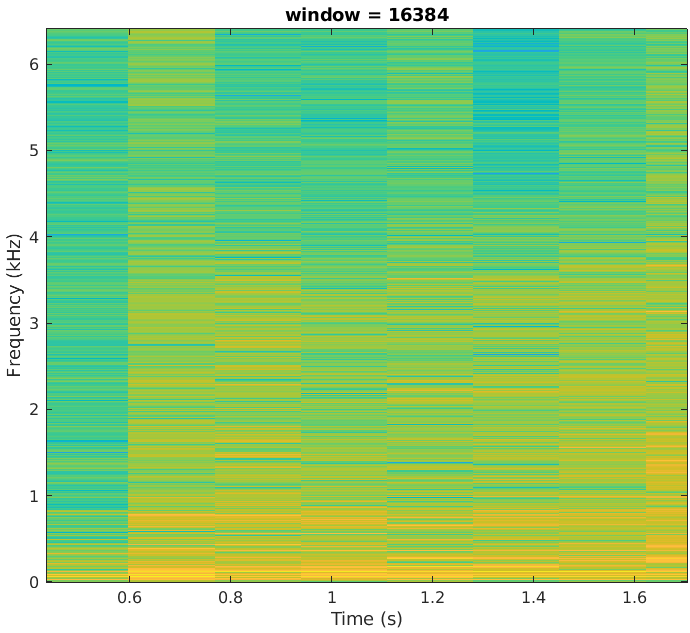
\includegraphics[width=5cm]{./stft_big_zoomed.png} }}
		\caption{STFT, small vs. big window}
	\end{figure}
\end{frame}

\begin{frame}
	\frametitle{STFT with gausswin (i.e. Gabor transform)}
	\begin{figure}
		\centering
		\subfloat[Gausswin]{{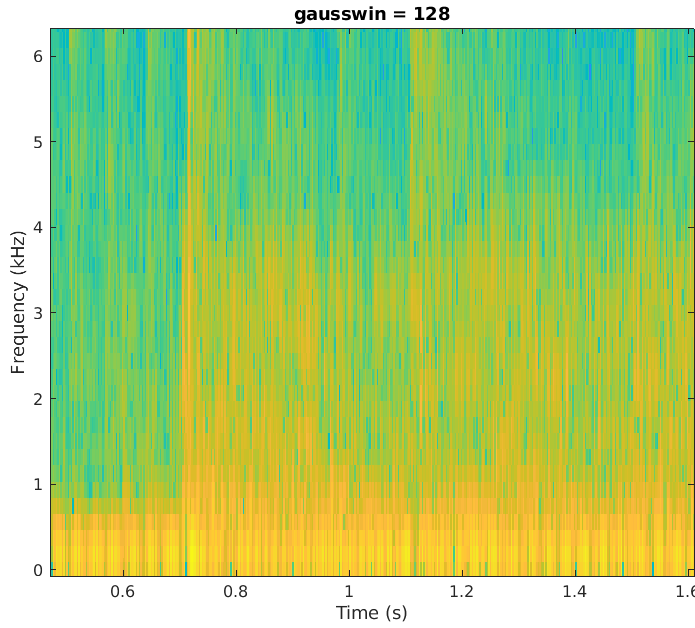
\includegraphics[width=5cm]{./gaborstft_small_zoomed.png} }}
		\subfloat[Hamming]{{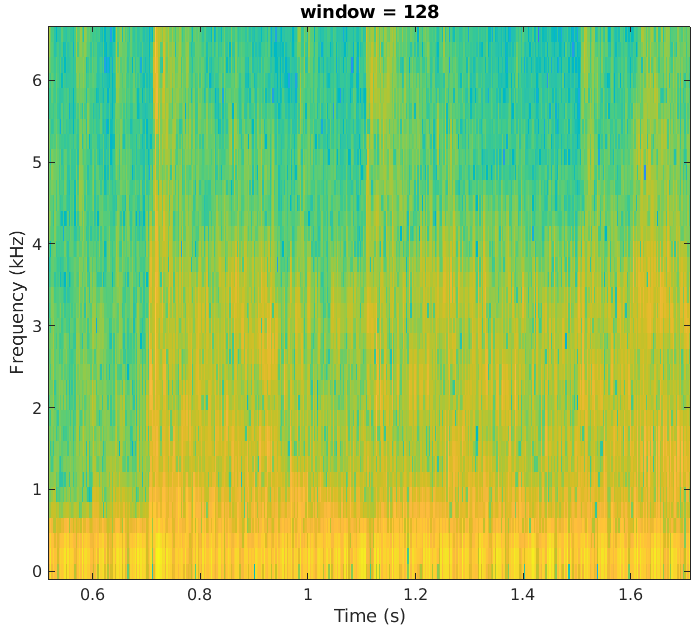
\includegraphics[width=5cm]{./stft_small_zoomed.png} }}
		\caption{STFT, small window = 128, Gaussian vs. Hamming}
	\end{figure}
\end{frame}

\begin{frame}
	\frametitle{STFT with gausswin (i.e. Gabor transform)}
	\begin{figure}
		\centering
		\subfloat[Gausswin]{{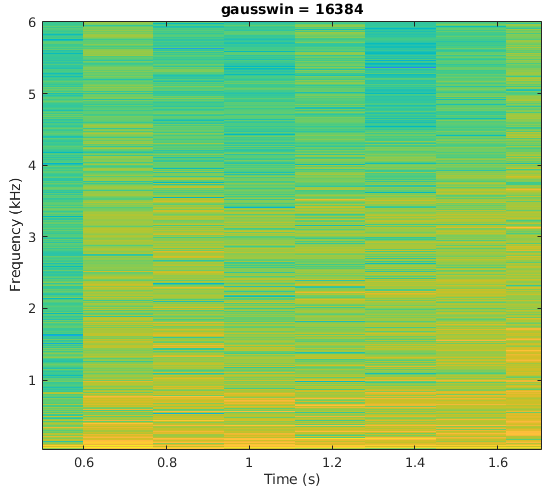
\includegraphics[width=5.2cm]{./gaborstft_big_zoomed.png} }}
		\subfloat[Hamming]{{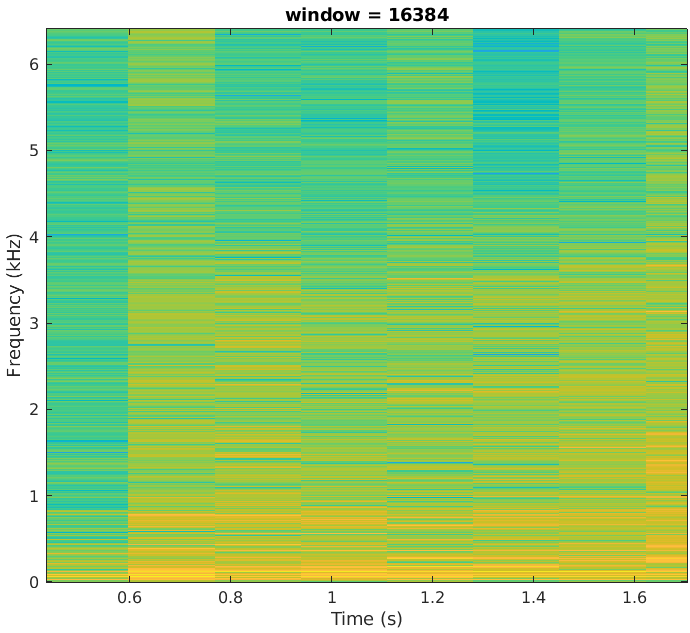
\includegraphics[width=5cm]{./stft_big_zoomed.png} }}
		\caption{STFT, large window = 16384, Gaussian vs. Hamming}
	\end{figure}
\end{frame}

\end{document}
